27. $\cfrac{(x^2-6x+8)(x^2-4)}{x^3+8}\geqslant0\Leftrightarrow \cfrac{(x-4)(x-2)^2(x+2)}{(x+2)(x^2-2x+4)}\geqslant0.$ Применив метод интервалов, найдём ответ: $x\in\{2\}\cup[4;+\infty).$
\begin{figure}[ht!]
\center{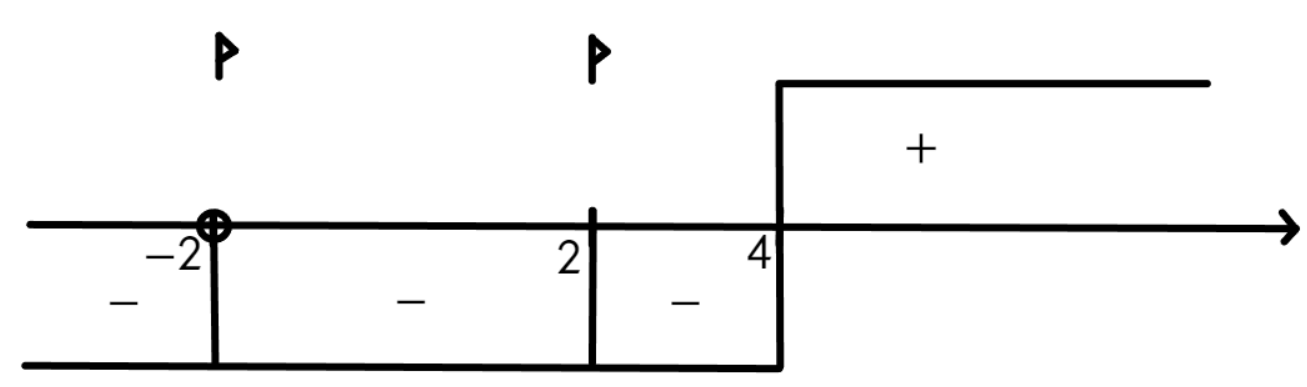
\includegraphics[scale=0.35]{ner9-27.png}}
\end{figure}\\
